%\subsection{Tapered waveguide due to taper length}
%tapered_length
The value of the divergence angle is also a important character of the tapered waveguide to determine the coupling ability. The author of \cite{study_linear_tapered_waveguides} has presented that the smaller the divergence angle is, the more power of fundamental mode propagates in the taper. In order to simplify the modeling process the variation of taper length will be performed in the following coupling simulations to discuss the effect of the divergence angle.
We will keep the taper interface width of the waveguide as a constant of $2\mu$m and change the taper length from $2\mu$m to $5.5\mu$m in following simulations.\\
  
\begin{figure}[!ht]
\centering
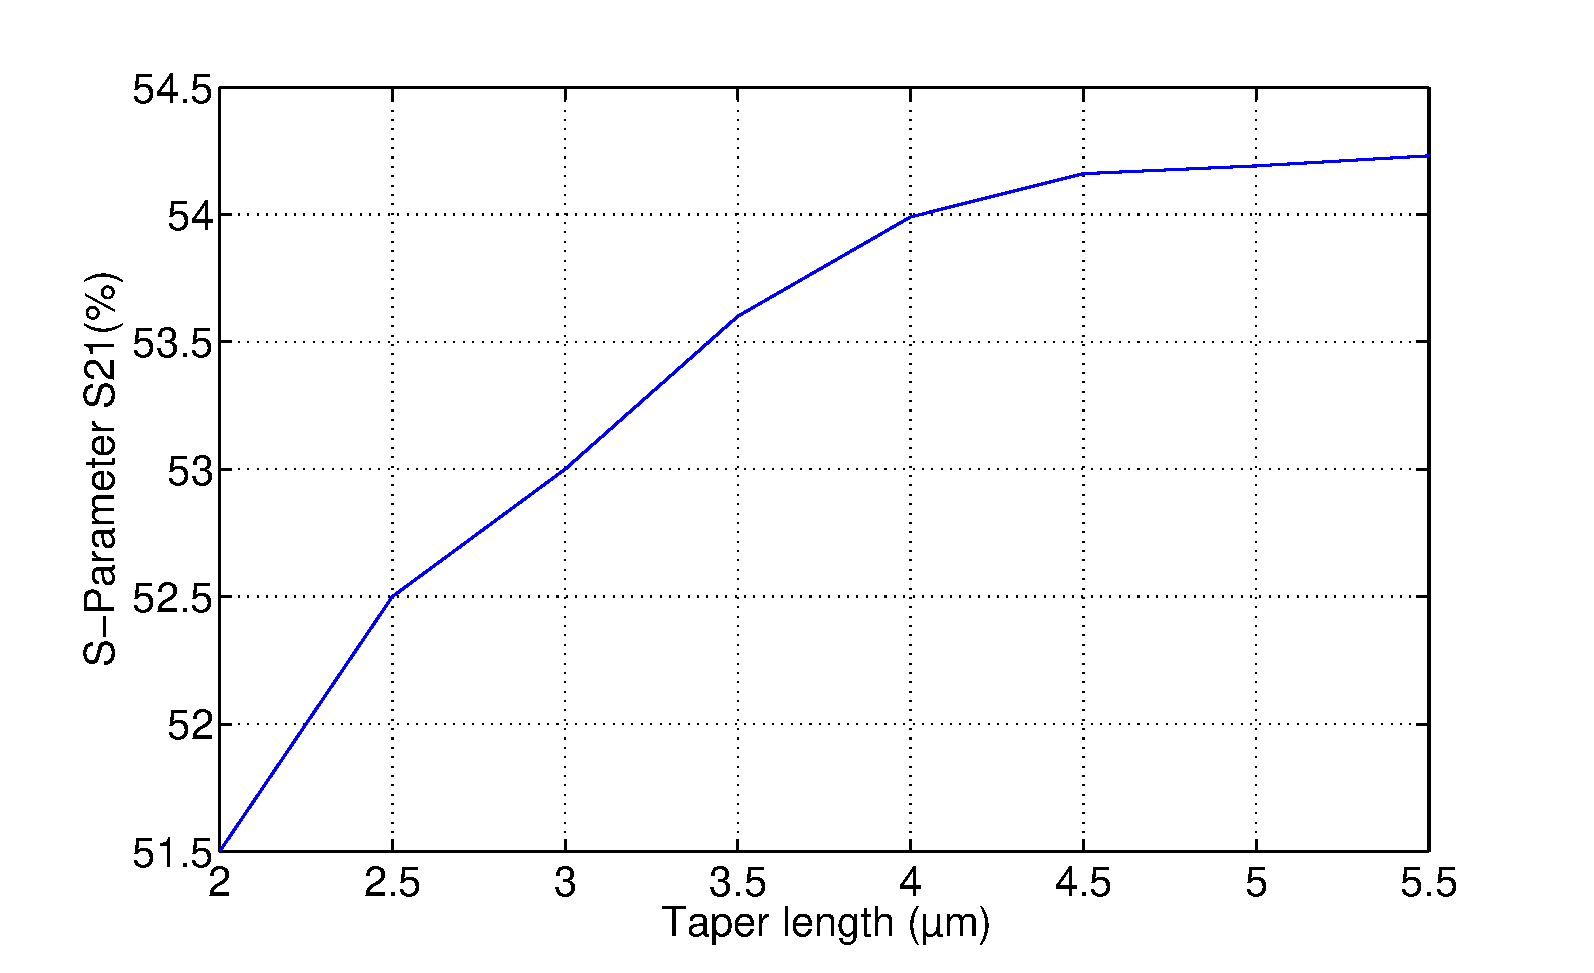
\includegraphics[width=0.7\textwidth]{bilder/tapered_waveguide_dxx}
\caption{Coupling efficiency between TLF and tapered waveguide due to taper length and taper width $= 2\mu$m.}
\label{fig:tapered_waveguide_dxx}
\end{figure}
The coupling behavior of the arrangement, the taper length vary from $2\mu$m to $5.5\mu$m, is shown in Fig. \ref{fig:tapered_waveguide_dxx}.  The figure illustrate that the coupling efficiency increase monotonously with the taper length expanding. After taper length $4.5\mu$m of the coupling efficiency rise more and more gently, close approximately to a constant $54\%$. 
Therefore for an efficient coupling the optimal divergence angle of the taper in this arrangement is less than:
\begin{equation}
\theta=atan\frac{d_{1}-d_{0}}{L_{taper}}=actan\frac{2-1}{5.5}=10.3^{o}
\label{eq:divergence_angle}
\end{equation}
